\chapter{Task 18: Turing Patterns}

\section{Task Description}
The goal of this task is to simulate a Turing activator-inhibitor dynamics on networks, possibly replicating some of the results reported in \cite{main_network}. 
\section{Mathematical Model}
An activator-inhibitor system on a network can be defined in very close analogy to what one does on a continuous medium. 
The equations for the system are of the reaction-diffusion type:
$$
\begin{cases}
\dot{u}_i(t) = f(u_i\, v_i) - \epsilon\,[L\,u(t)]_i \\
\dot{v}_i(t) = g(u_i\, v_i) - \epsilon\, \sigma [L\,v(t)]_i \\
\end{cases}
$$
Here, $\mathbf{u} = (u_1, \cdots u_N)$ and $\mathbf{v} = (v_1, \cdots v_N)$ are, respectively, the concentrations of the activator and the inhibitor substance on the $N$ nodes of the network. The reactions take place on each node and are encoded in the reaction terms $f$ and $g$. L is the laplacian matrix, defined as $L=D-A$ where $D_{i,\,j}=k_i \cdot \delta_{i,j}$ and $A$ is the adiacency matrix. The diffusivity of the activator substance is $\epsilon$, while that of the inhibitor is $\epsilon\,\sigma$, so that $\sigma$ is the ratio between them. The reaction terms are supposed to satisfy two basic requirements:
\begin{enumerate}
	\item There exists a homogeneous equilibrium $(\overline{u},\, \overline{v})$ which is linearly stable in the absence of diffusion (indeed, the key concept of the Turing model is that the instability is driven by diffusion). In mathematical terms [Appendix: \ref{app:bifurcation_diagram}]:
\begin{equation}
\begin{pmatrix}
    f(\overline{u}\,, \overline{v}) \\
    g(\overline{u}\,, \overline{v}) 
\end{pmatrix}
= 
\begin{pmatrix}
    0 \\
    0 
\end{pmatrix}
\quad \text{and} 
            \quad
 		\begin{cases}
 			\text{tr}(J)= f_u + g_v < 0\\
 			\text{det}(J) = f_u\cdot g_v f_v\cdot g_u>0
 		\end{cases},\,
      J(\overline{u}\,, \overline{v}) := 
		\begin{pmatrix}
 			f_u & f_v \\
 			g_u & g_v
 		\end{pmatrix}
  \label{eq:basic_1}
\end{equation}
	
	\item Correct qualitative behaviour of reactions in the neighborhood of the fixed point $(\overline{u},\, \overline{v})$: the activator $u$ is supposed to enhance its own production and the production of the inhibitor $v$. Viceversa, the inhibitor $v$ is supposed to suppress the production of both the activator $u$ and itself. The functions $f,\, v$ need to reflect this behaviour, at least in a neighbourhood of the equilibrium $(\overline{u},\, \overline{v})$.In mathematical terms:
    \newline
        \begin{minipage}{0.48\textwidth}
    \centering
	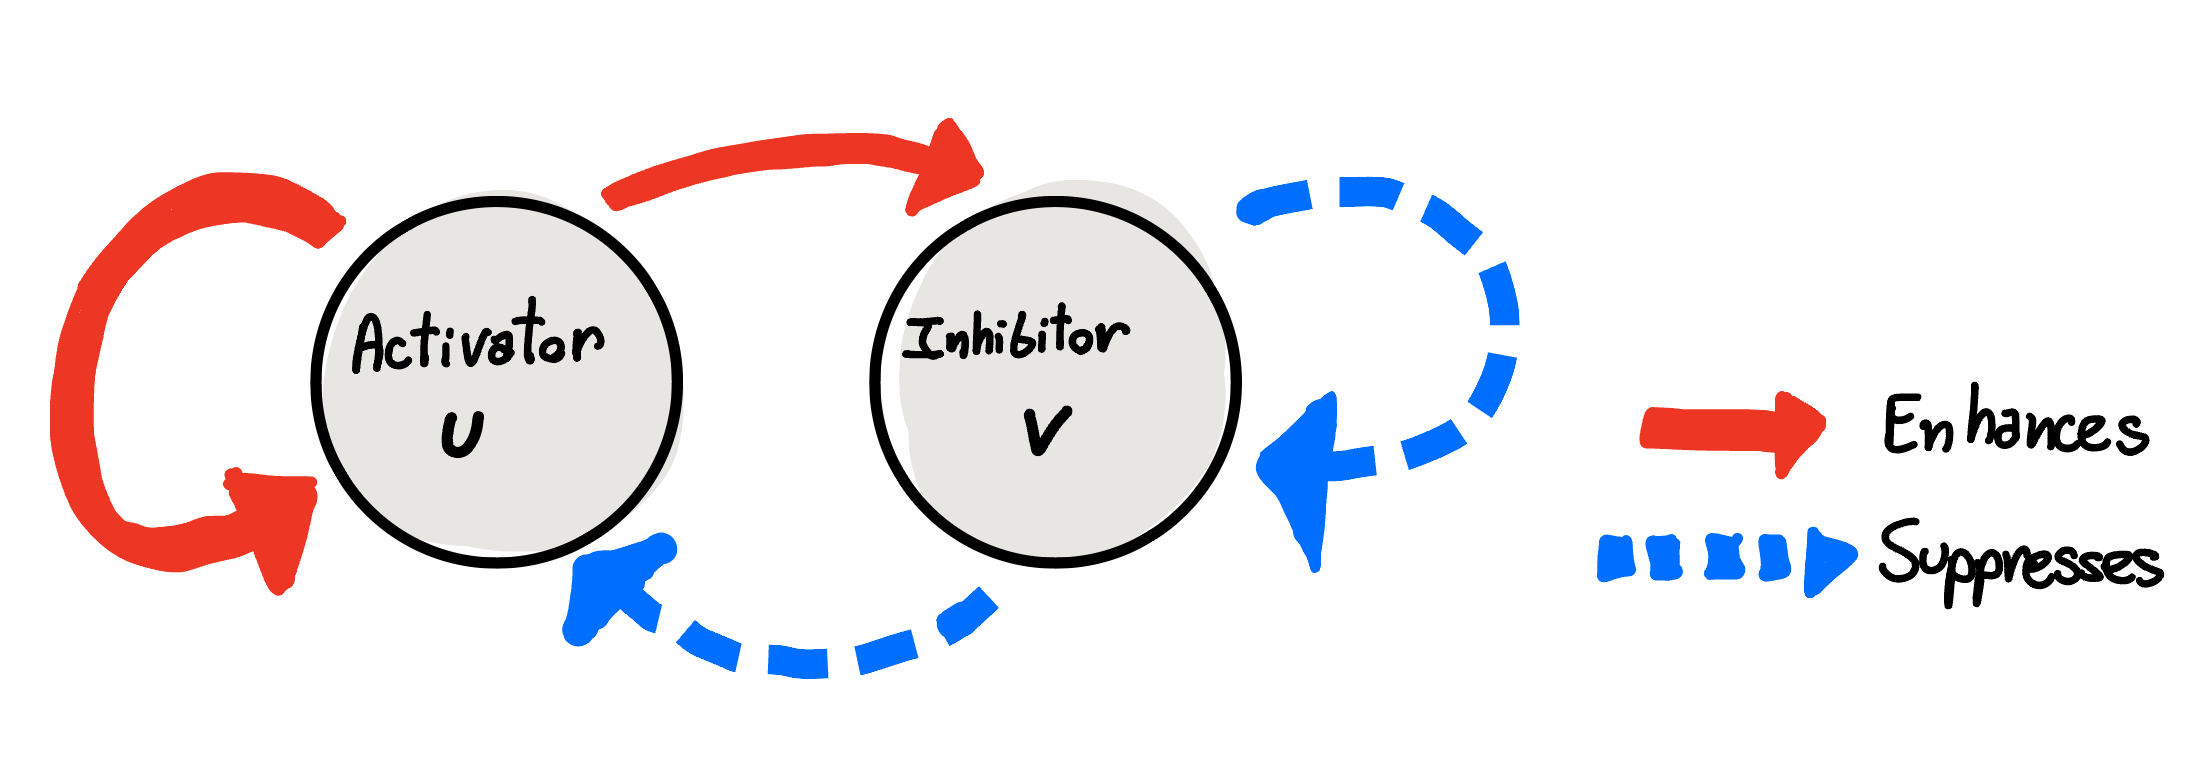
\includegraphics[width=\textwidth]{images/turing/diagram.jpeg}
 \label{fig:diagram}
    \end{minipage}
    \hfill
    \begin{minipage}{0.4\textwidth}
    \centering
    \begin{equation}
           \begin{cases}
         f_u > 0,\quad f_v < 0 \\
         g_u >0,\quad  g_v <0 \\      
        \end{cases} 
        \label{eq:basic_2}
        \end{equation}
    \end{minipage}
\end{enumerate}
The conditions for pattern emergence are found through linear stability analysis of the uniform stationary state $(\overline{u},\,\overline{v})$ with respect to the perturbation. The perturbation is expanded in the ortonormal basis of the laplacian eigenvectors $\{\Phi^{(n)}\}_{n=1}^{N}$:
\begin{equation*}
    \begin{pmatrix}
    \delta u_i (t) \\
    \delta v_i (t) \\
    \end{pmatrix}
    =
    \begin{pmatrix}
        1 \\
        B_n \\
    \end{pmatrix}
    \cdot \sum_{n=1}^{N}\, c_n\,\Phi_i^{(n)}\, e^{\lambda_n\,t} \\
\end{equation*}
where coefficients $c_n$ are determined by the initial conditions. The growth rate $\lambda_n$ of the $n-$mode is found through the resolution of an eigenvalue problem that depends on $(\Lambda_n, \sigma$, $\epsilon)$, where $\Lambda_n$ is the laplacian eigenvalue associated with eigenvector $\Phi^{(n)}$. The function $\mathcal{R}e\{\lambda_n\} (\Lambda_n | \epsilon, \sigma)$ is usually referred to as the \textit{dispersion relation}.
Whether the $n$-mode amplitude grows with time or decays depends on the sign of $\mathcal{R}e\{\lambda_n\}$. One finds that the dispersion curve $\mathcal{R}e\{\lambda\}(\Lambda|\epsilon, \sigma)$ lies entirely below the x axis for $\sigma < \sigma_C$ ($\Rightarrow$ no instability), while assumes positive values in some range of positive $\Lambda$'s for all $\sigma > \sigma_C$ ($\Rightarrow$ instability). This critical threshold $\sigma_C$ is a function of the jacobian $J$ [Eq: \ref{eq:basic_1}] alone:
\begin{equation}
 \sigma > \sigma_c :=  \frac{(f_u\,g_v - 2\,f_v\,g_u)\, + 2\,\sqrt{f_v\,g_u\,(f_v\,g_u-f_u\,g_v))}}{f_u^2}
 \label{eq:critical_threshold}
\end{equation}
and always satisfies $\sigma_C > 1$, i.e. the diffusivity of the inhibitor substance is higher than that of the activator (this is in fact the key reason why the diffusion process can induce patterns: see Appendix figure \ref{fig:key} for discussion). \newline \noindent
For $\sigma$ slightly above the critical threshold, the unstable mode(s) will correspond to eigenvalues $\Lambda_n$ located closely around the \textit{critical eigenvalue}
\begin{equation}
    \Lambda_c(\epsilon) := \frac{1}{\epsilon}\,\sqrt{\frac{\text{det}[J]}{\sigma_c}}
    \label{eq:critical_eigenvalue}
\end{equation}
The full derivation of the above equations [Eq: \ref{eq:critical_eigenvalue}, \ref{eq:critical_threshold}] is presented in [Appendix: \ref{section:conditions_for_instability}].
The subsequent evolution of the pattern is non-linear and eventually results in a steady state (that can be either stationary or time dependent).  \bigskip \newline \noindent
\section{Numerical Simulations}
As in \cite{main_network}, the reaction terms are set as
\begin{equation}
    \begin{cases}
        f(u,v) = [\frac{a + b\,u -u^2}{c} - v]\, u \\
        g(u, v) = [u - (1+ d\,v)]\cdot v 
    \end{cases}
\label{eq:chosen_kinetics}
\end{equation}
with parameters $a\,=\,35,\, b=16,\, c= 9,\, d= 2/5$, 
helding a linearly stable fixed point $(\overline{u},\, \overline{v}) = (5, 10)$ and a critical diffusion ratio $\sigma_c \simeq 15.5$. \newline \noindent
\begin{figure}[H]
    \centering
    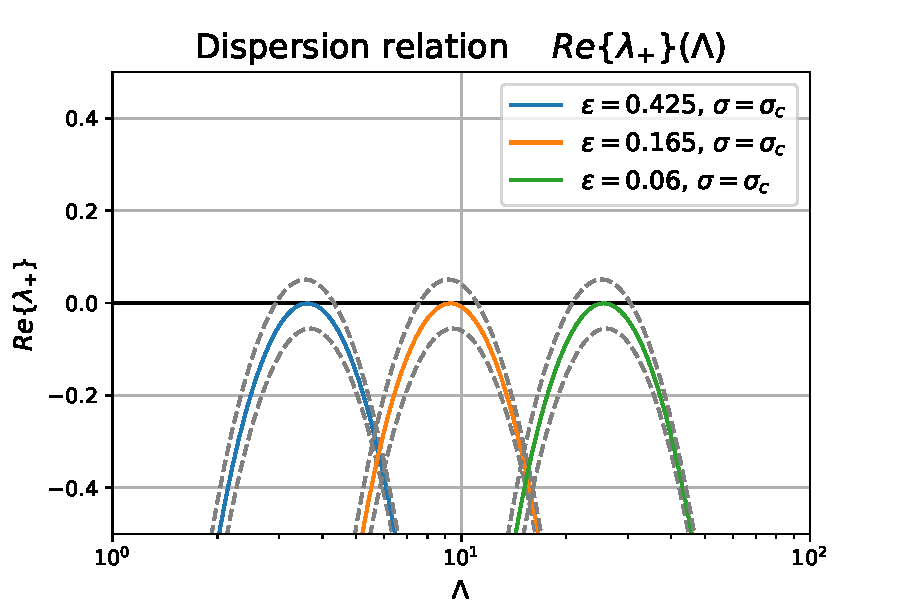
\includegraphics[width=0.7\textwidth]{latex_source/images/turing/multiple_dispersion.pdf}
    \caption{ Dispersion relation for the chosen reaction kinetics [Eq. $\ref{eq:chosen_kinetics}$], at different values of the activator diffusivity $\epsilon$. The dashed grey lines are the dispersion curves slightly above and below the critical diffusivity ratio $\sigma_c$. The critical eigenvalue $\Lambda_c$ [Eq. \ref{eq:critical_eigenvalue}] is inversely proportional to the activator diffusivity $\epsilon$.}
\end{figure}
Following the choice of the authors, I simulated the dynamics on Barabasi-Albert scale free networks. I chose parameters $N = 200$ for the number of nodes and $\left \langle k \right \rangle = 10$ for the mean degree. My activator diffusivity was $\epsilon = 0.12$, and my diffusivity ratio was $\sigma = 15.6 > \sigma_c = 15.5$. The reasoning for chosing a diffusivity ratio that is only slightly above the critical threshold is to keep the number of different allowed modes low.
\begin{figure}[H]
\centering
\subfigure[]{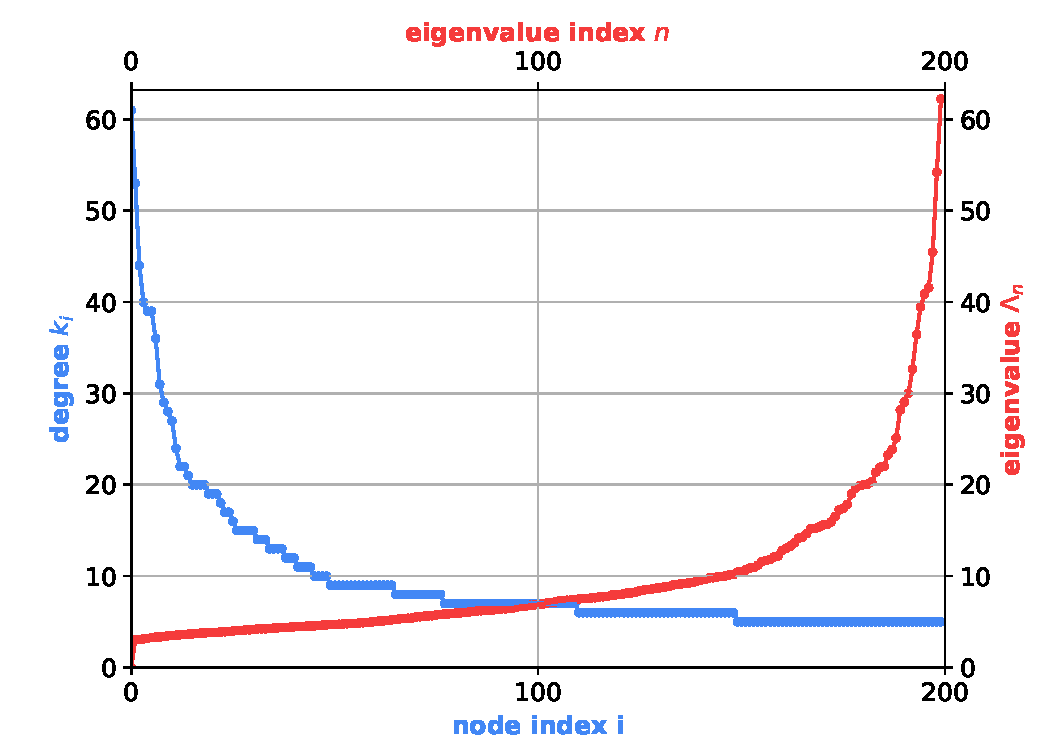
\includegraphics[width = 0.47\textwidth]{latex_source/images/turing/network_200.pdf}}
\hfill
\subfigure[]{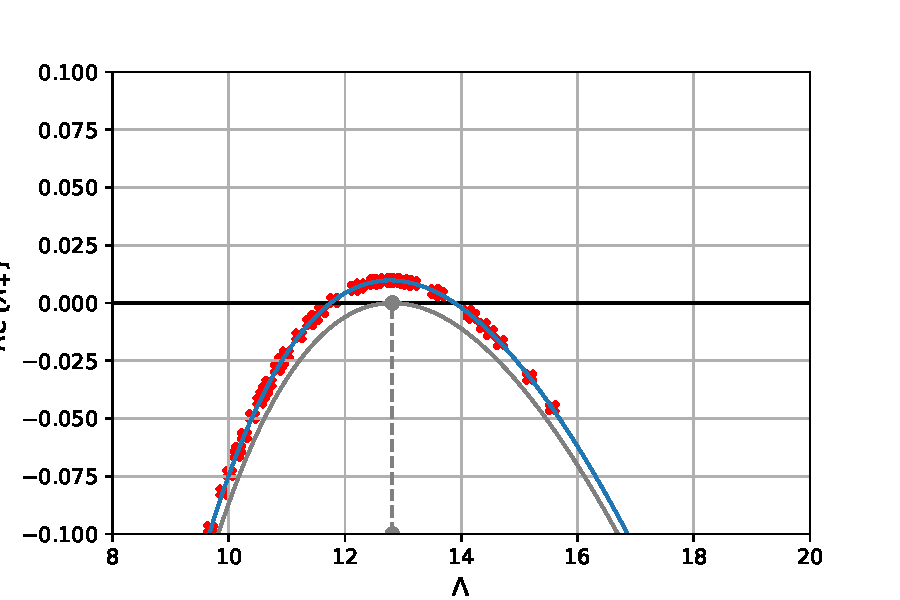
\includegraphics[width = 0.47\textwidth]{latex_source/images/turing/simulation_dispersion.pdf}}
\caption{ Most relevant properties of the network used in the simulation. Subfigure (a) shows the degree spectrum and the laplacian eigenvalue spectrum of the chosen graph. Network nodes are indexed by decreasing degree. Subfigure (b) shows the dispersion relation curve. Critical eigenvalue is $\Lambda_c \simeq 12.8141$. The eigenvalue closest to $\Lambda_c$ is $\Lambda_n \simeq 12.64$, of index $n=157$. However, as one can see from the graph, the network eigenvalue spectrum comprehends several other allowed modes (red crosses) in the unstable range, and they are expected to contribute to pattern initiation as well.}
\end{figure}
\noindent
The initial homogeneous state $(\overline{u},\,\overline{v})$ was perturbed with a random uniform perturbation at each node of amplitude $0.05$. [Figure \ref{fig:snapshots}] show snapshots of the activator concentration on nodes at different times. Also, the GithHub repository \cite{git} contains a .mp4 video of the whole evolution. 
\begin{figure}[H]
    \centering
    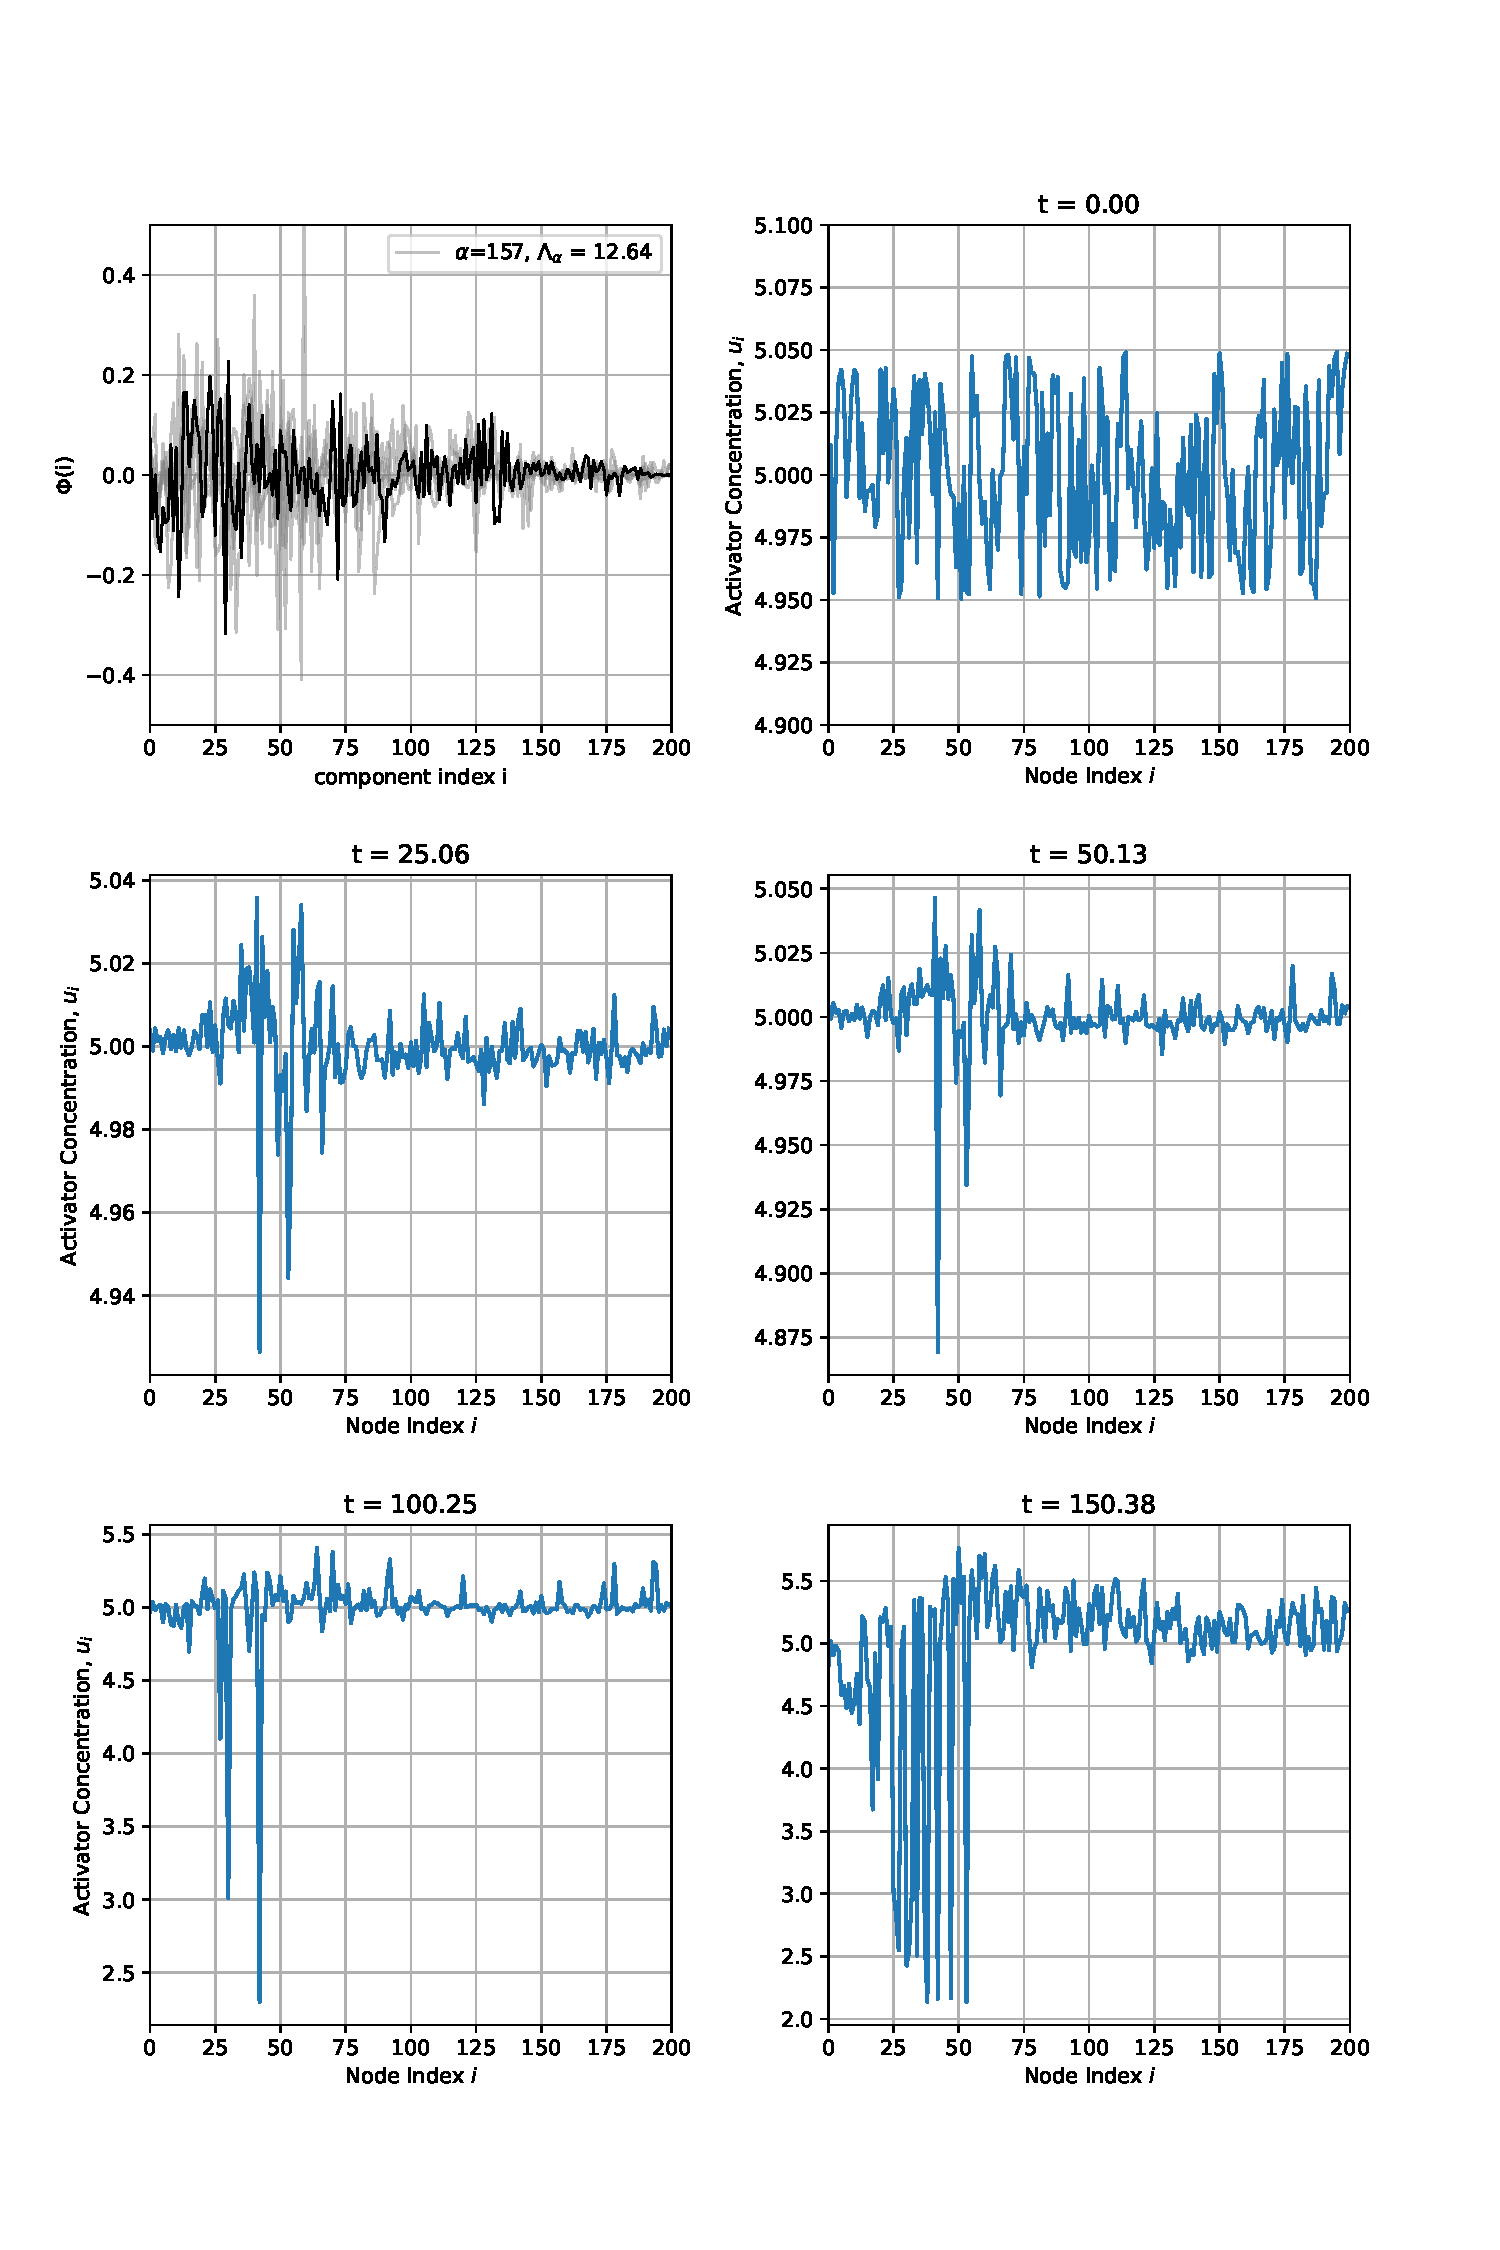
\includegraphics[width = 0.81\textwidth]{latex_source/images/turing/snapshots.pdf}
    \caption{ Time evolution of the activator concentration. The subfigure at top left corner shows the components of the critical eigenvector (black) and its closest neighbours in the unstable range (grey).}
    \label{fig:snapshots}
\end{figure}
In the early stage, the pattern is expected to grow proportionally to the critical eigenvector, which is is the mode of largest growing rate: $\delta\,u(t),\, \delta\,v(t) \propto \Phi^{(n)}$.
In fact, when the initial uniform perturbation dies out and the pattern starts to grow, the activator substance distribution is located similarly to the critical eigenvector (see snapshot $t = 25.06$). Later on, the evolution becomes strongly non-linear and the pattern is reshaped (see snapshot at $t = 100.25$), till it settles into a stationary state (see snapshot at $t = 150.38$) where nodes are split into one activator-rich group and one activator-poor group. The authors found that this peculiar behaviour is well described in the framework of a mean field theory \cite{main_network}. \medskip \newline \noindent
One thing that can be noticed in the initial stage pattern [Figure \ref{fig:snapshots}, snapshot at $t = 25.06$] is that the significant variations of the activator level are localized on a subset of nodes of close degree ($k \sim 25-75$). That is, only a specific subset of the network undergoes differentiation. This effect is was not a fortuity but is due to the fact that the laplacian eigenvectors in a large graph with a broad degree distribution tend to be localized around a specific degree $\overline{k}(\Lambda)$. Also, as authors report, a simple relation $\overline{k}(\Lambda) \simeq \Lambda$ seems to hold. I checked wether I could find the same behaviour for my graph (see [Figure \ref{fig:eigenvectors}] and [Figure \ref{fig:heatmap}]).
\begin{figure}[H]
\centering
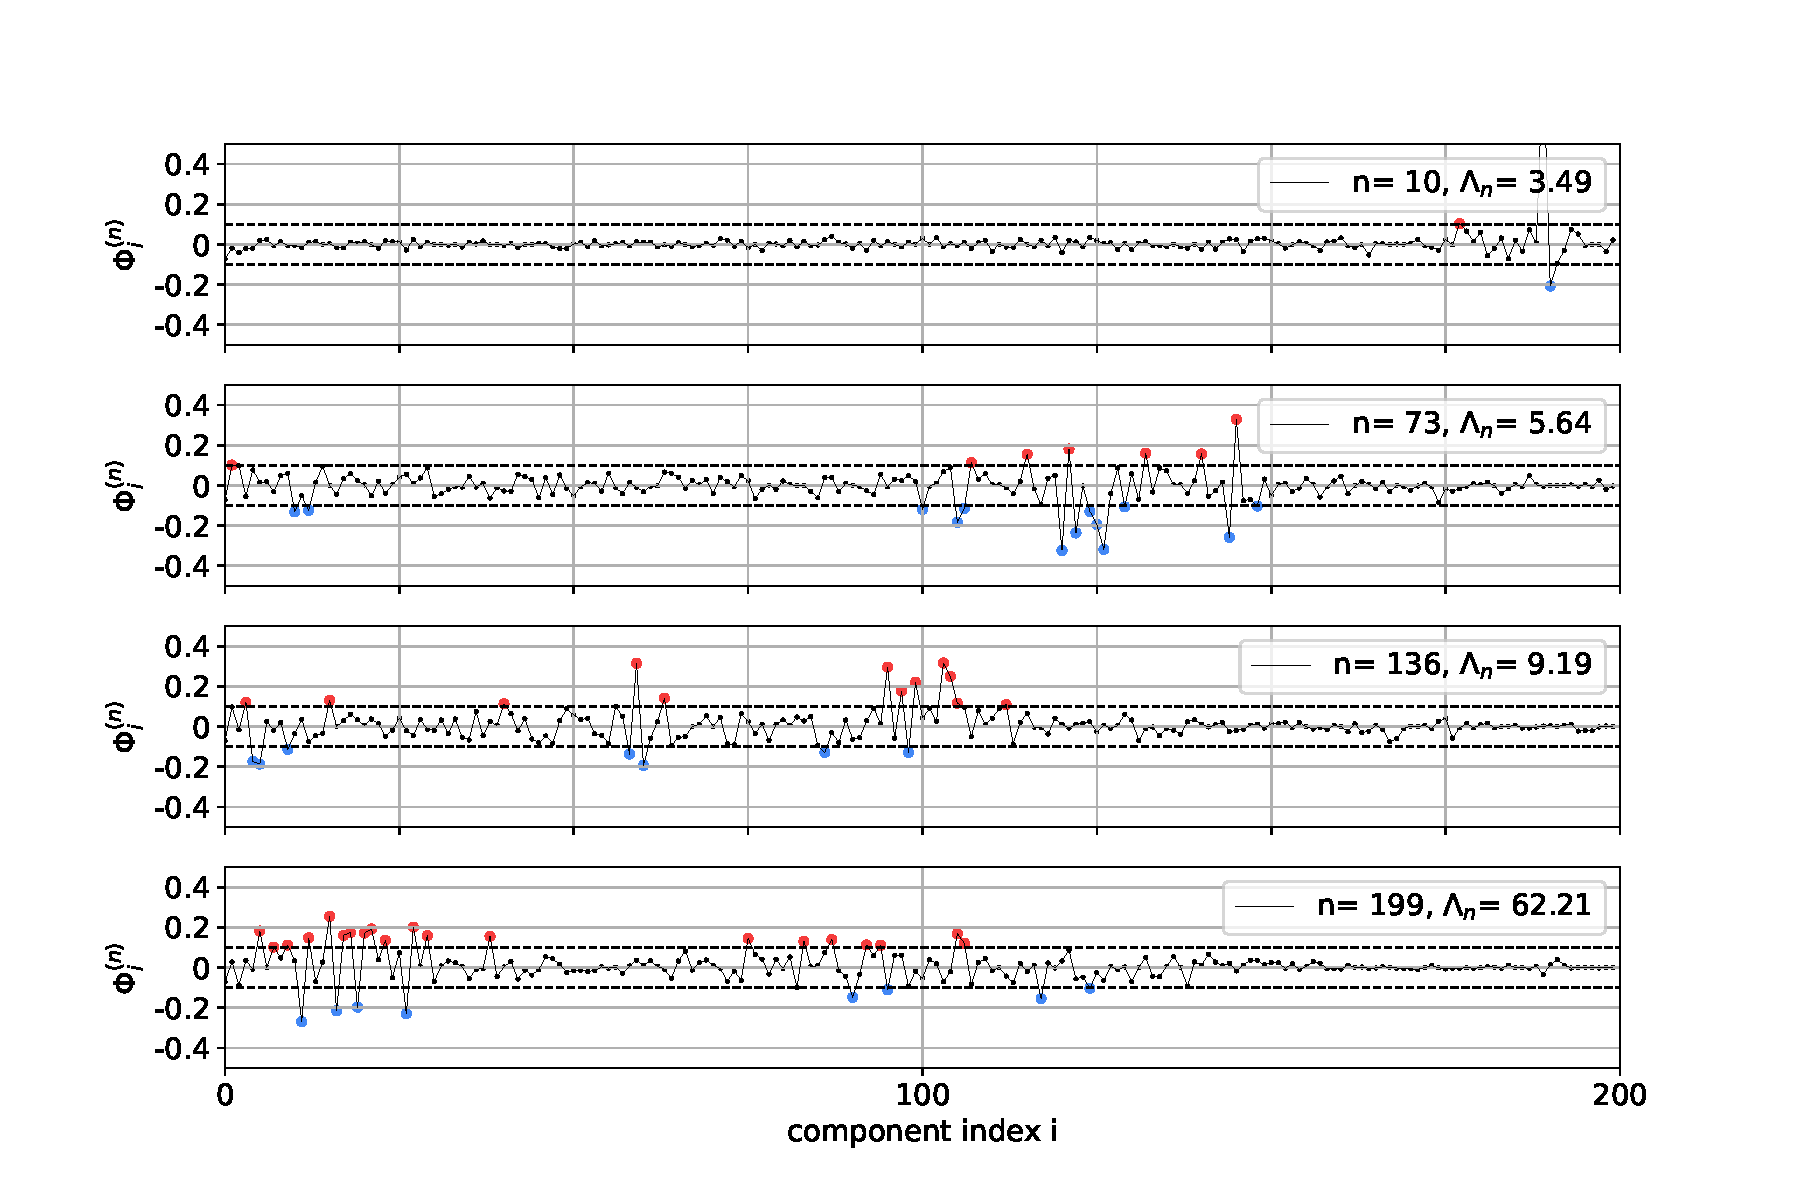
\includegraphics[width =\textwidth]{latex_source/images/turing/eigenvectors_200.pdf}
\caption{Localization of laplacian eigenvectors in 
a BA with $N=200$ and $\left \langle k \right \rangle = 10$. Nodes nodes are ranked by their degree. With incrementing eigenvalue $\Lambda$, the characteristic degree becomes higher.}
\label{fig:eigenvectors}
\end{figure}

\begin{figure}[H]
    \centering
\subfigure[]{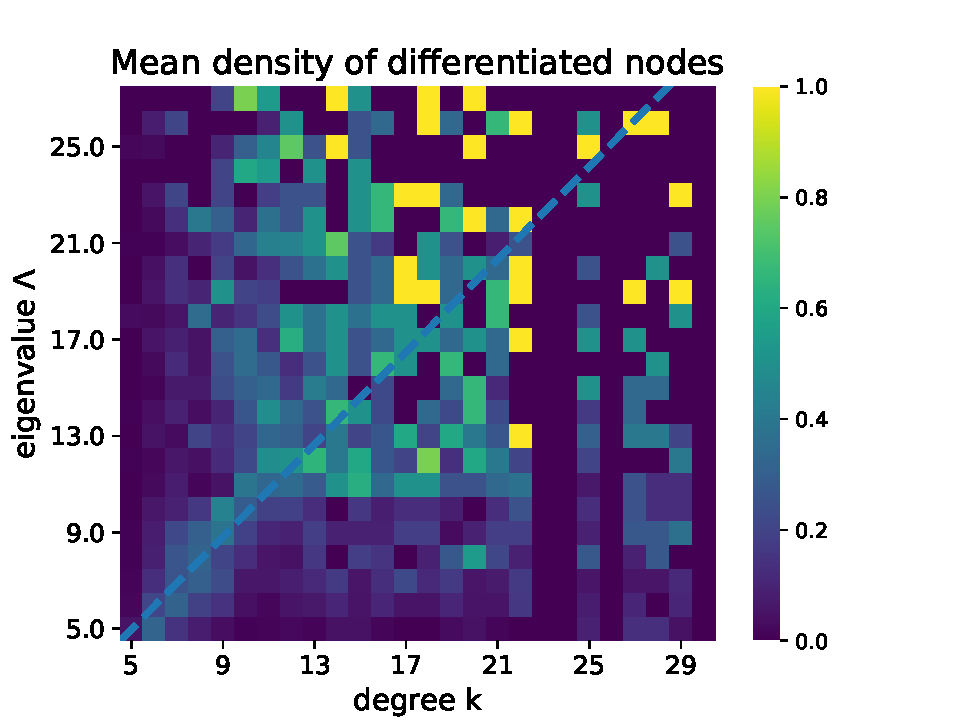
\includegraphics[width=0.48\textwidth]{latex_source/images/turing/density_200.pdf}}
\subfigure[]{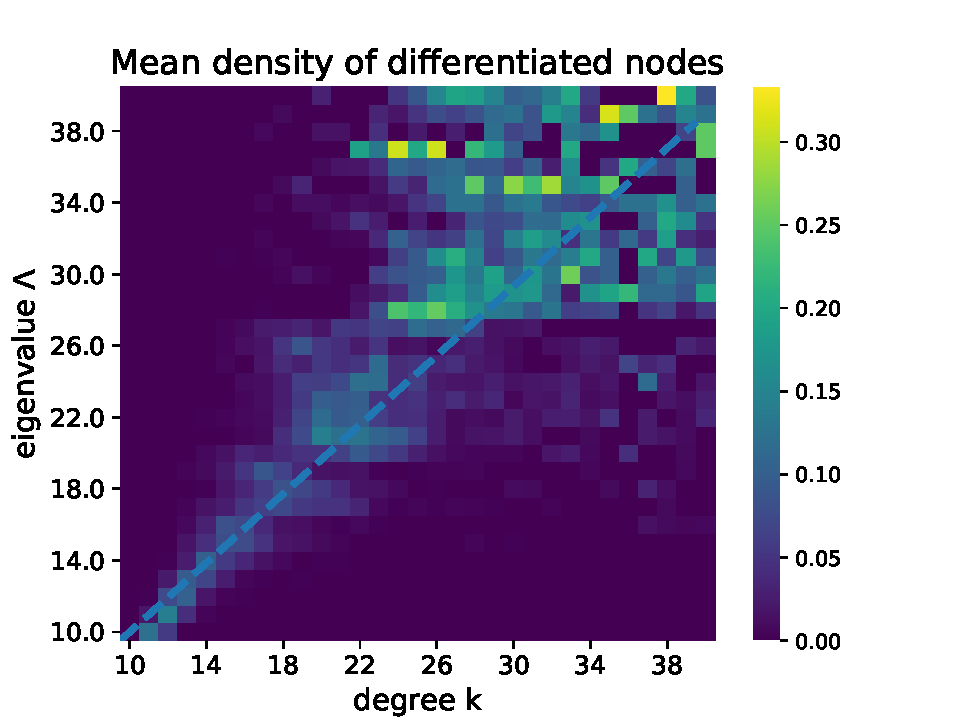
\includegraphics[width=0.48\textwidth]{latex_source/images/turing/density_1000.pdf}}
\caption{Localization of laplacian eigenvectors in a BA graph with $N=200$ nodes and $\left \langle k\right \rangle=10$ (a) and in a BA graph with $N=1000$ nodes and $\left \langle k \right \rangle=20$ (b). Eigenvalues have been grouped into bins of unitary width. The population of nodes inside each degree group, $N_k$, was calculated. The heatmap represents the mean density of differentiated nodes for each degree group $z = N_k^{\text{diff}}(\Lambda)/N_k$. A node $i$ of degree was considered to be differentiated with respect to eigenvalue $\Lambda_n$ if its eigenvector component satisfied, $|\Phi_i^{(n)}|> 0.1$. I found, like authors \cite{main_network} report, that approximately $\overline{k}(\Lambda) \propto \Lambda$ (dashed line) and that effect is more pronounced in the larger graph.}
\label{fig:heatmap}
\end{figure}

\nocite{bio_article}
\nocite{murray}
\nocite{altbook}
\newpage
\section*{Appendix}
\addcontentsline{toc}{section}{Appendix}
\subsection*{Linear Stability of a 2x2 autonomous system}
\label{app:bifurcation_diagram}
{\small
Say $(\overline{x},\, \overline{y})\in \mathbbm{R}^2$ is a fixed point (or equilibrium) of the autonomous system 
\begin{equation*}
    \begin{pmatrix}
        \dot{x}(t) \\
        \dot{y}(t) \\
    \end{pmatrix}
    = 
        \begin{pmatrix}
        f[x(t),\, y(t)] \\
        g[x(t),\, y(t)] \\
    \end{pmatrix}
\end{equation*}
which, namely, means that $f(\overline{x},\, \overline{y}) = g(\overline{x},\, \overline{y}) = 0$. Now we want to study how the system evolves if a small perturbation $(\delta x,\, \delta y)$ is added to the equilibrium. We can linearize the system:
\begin{equation*}
    \begin{pmatrix}
        \delta\,\dot{x}(t) \\
        \delta\,\dot{y}(t) \\
    \end{pmatrix}
    = 
        \begin{pmatrix}
        \frac{\delta\,f}{\delta x}|_{(\overline{x},\,\overline{y})} & \frac{\delta\,f}{\delta y}|_{(\overline{x},\,\overline{y})}\\
        \frac{\delta\,g}{\delta x}|_{(\overline{x},\,\overline{y})} & \frac{\delta\,g}{\delta y}|_{(\overline{x},\,\overline{y})} \\
    \end{pmatrix}
    \cdot
        \begin{pmatrix}
        \delta\,x(t) \\
        \delta\,y(t) \\
    \end{pmatrix}
    +
    o(||(\delta\,x, \delta\,y)||)
\end{equation*}
 The latter is a homogeneous linear system with general solution:
\begin{equation*}
        \begin{pmatrix}
        x(t) \\
        y(t) \\
    \end{pmatrix}
     = 
     \alpha_1 \mathbf{v}_1\, e^{\lambda_1\, t} + \alpha_2 \mathbf{v}_2\, e^{\lambda_2\, t} 
\end{equation*}
where $\lambda_1,\, \lambda_2$ are the eigenvalues of the jacobian and $\mathbf{v}_1\, \mathbf{v}_2$ are the corresponding eigenvectors, and $\alpha_1, \alpha_2$ are coefficients determined by the initial condition. The eigenvalues of a $2\cdot 2$ matrix can be both real or complex cooniugates ($\lambda_1 = \lambda, \, \lambda_2 = \overline{\lambda}$). Wether the amplitude of the perturbation dies out exponentially or explodes depends on the sign of $\mathcal{R}e\{\lambda\}$. The linear stability requirement is
$$
\mathcal{R}e\{\lambda\} <0 \quad \text{for both} \, \lambda\text{'s}
$$
The eigenvalues $\lambda_1,\, \lambda_2$ are the roots of the characteristic polynomial of the jacobian $J$:
\begin{equation*}
    p_J(\lambda) = (\lambda - \lambda_1)\cdot (\lambda - \lambda_2) = \lambda^2 - \text{tr}[J]\cdot\lambda + \text{det}[J]
\end{equation*}
\begin{minipage}{0.4\textwidth}
Then we have the following cases, depending on the discriminant $\Delta^2 = \text{tr}[J]^2 - 4\,\text{det}[J]$:
\begin{equation*}
    \begin{cases}
        \Delta^2 > 0: \quad \lambda_1,\, \lambda_2  =  \frac{\text{tr}[J] \pm \Delta }{2} \\
        \Delta^2 = 0: \quad \lambda_1,= \lambda_2 = \frac{\text{tr}[J]}{2} \in \mathbbm{R} \\
        \Delta^2 <0: \quad \lambda_1,= \lambda_2  = \alpha \pm i \beta \in \mathbbm{C}
    \end{cases}
\end{equation*}
One can easily see from the polynomial $p_J(\lambda)$ that in the case $\Delta^2 \geq 0$, the requirement that both roots are negative is satisfied if and only if $\text{tr}[J]<0,\, \text{det}[J] >0$. In the case $\Delta <0$, we have obligatorily $\text{det}[J] = \lambda \cdot \overline{\lambda} = |\lambda|^2 >0$, and $\text{tr}[J]= 2\cdot \mathcal{R}e(\lambda)$. Then again the requirement holds if and only if $\text{tr}[J]< 0$.
\end{minipage}
\hfill
\begin{minipage}{0.5\textwidth}
\centering
    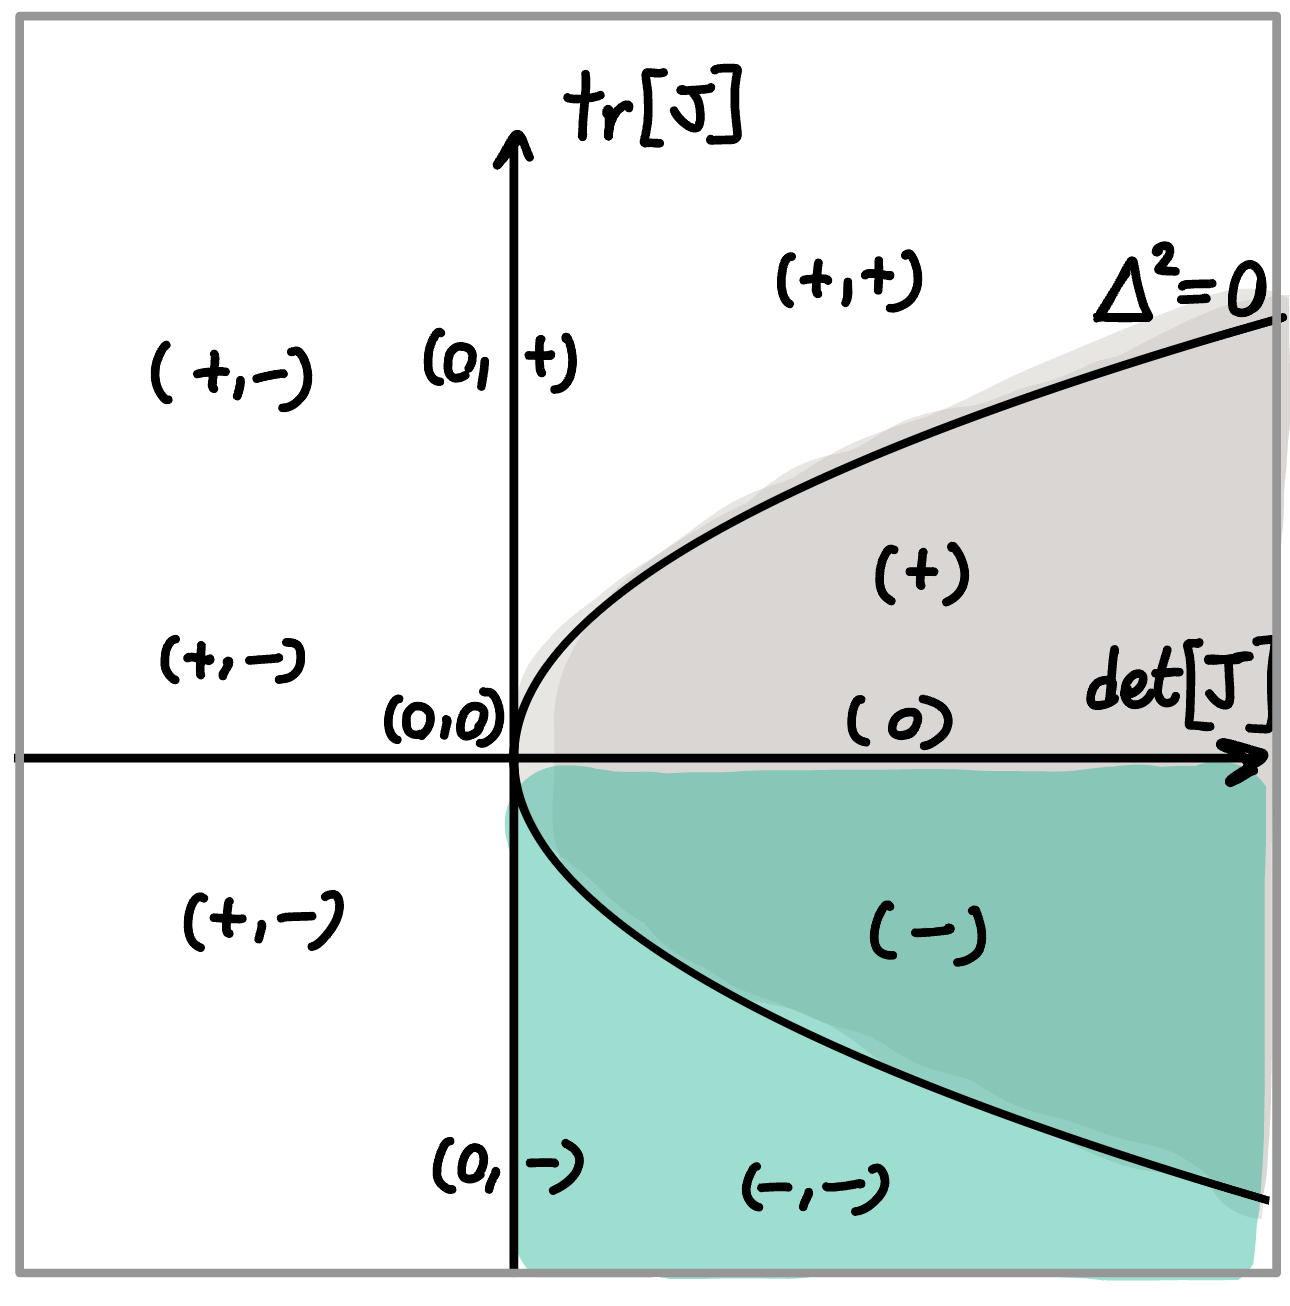
\includegraphics[width=0.8\linewidth]{latex_source/images/turing/bifurcation.jpeg}
    \captionof{figure}{Bifurcation diagram for a $2\cdot\,2$ homogeneous system. $(\pm,\,\pm)$ are the signs of $\mathcal{R}e\{\lambda\}$ in the various regions of the (tr[J], det[J]) plane. Green marks the stability region and grey marks the region where eigenvalues are complex.}
    \label{fig:bifurcation}
\end{minipage}
}
\bigskip \newline \noindent
\subsection*{An intuition of how diffusion can produce patterns}
[Figure \ref{fig:key}] can help understand how the activation - inhibition mechanism can induce the formation of heterogeneous patterns. Graph $1$ shows the initial condition of the system. Suppose that the concentration of the
activator is relatively higher than in other regions by random fluctuation. By the
self-enhancing property of the activator, the concentration of activator increases at the
center region (graph $2$), followed by the increase of inhibitor at the neighboring region A.
As the \textbf{diffusion rate of inhibitor is larger} than that of the activator, substantial
amounts of inhibitor move toward the lateral regions. This depresses the activator
function, resulting in the decrease of the activator concentration there (graph $3$).
Decrease of activator causes the decrease of inhibitor in the wider region (graph $4$). At
the region B, as inhibitor concentration is gotten lower, activator becomes relatively
dominant than inhibitor. This situation is enough to start the local self activation at
region B (graph $5$). 
\begin{figure}[H]
    \centering
    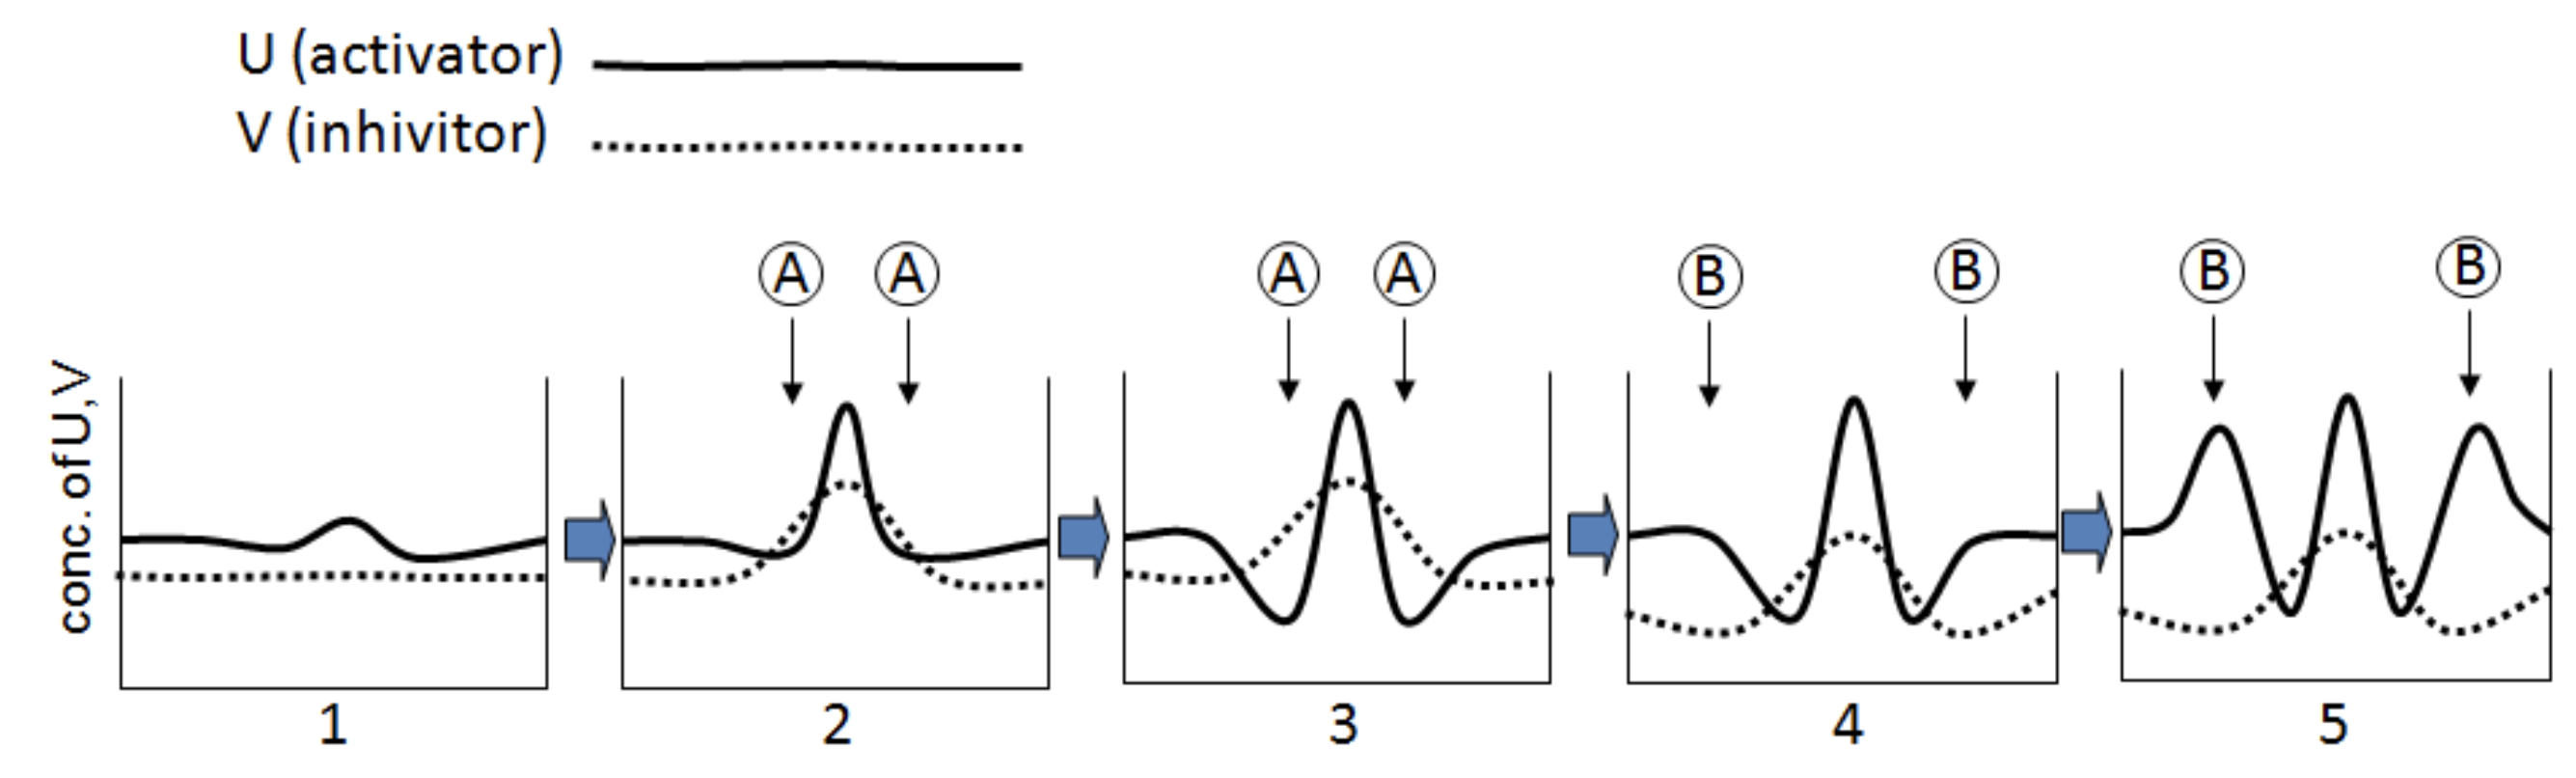
\includegraphics[width=0.8\linewidth]{latex_source/images/turing/key_mechanism.png}
    \label{fig:key}
    \caption{ Picture taken from \cite{bio_article}.}
   \label{fig:key}
\end{figure}

\subsection*{Conditions for diffusion-driven instability}
\label{section:conditions_for_instability}
{ \small
Diffusion driven instability is investigated by means of linear stability analysis. A small random perturbation $\delta\,u_i,\, \delta\,v_i$ is added at each node, starting from the homogeneous equilibrium state. A linearized system of equations is obtained for the evolution of the perturbation:
\begin{equation*}
    \begin{cases}
    u_i(t) = \overline{u} + \delta\, u_i(t)\\
    v_i(t) = \overline{v} + \delta\, v_i(t)
    \end{cases}
    \rightarrow 
    \begin{cases}
    \delta\, \dot{u}_i(t) \simeq \quad     f_u\, \delta u_i(t) +  f_v\, \delta v_i(t) - \epsilon\,[L\cdot (\overline{u}+ \delta u(t))]_i\\
    \delta\, \dot{v}_i(t) \simeq \quad 
    g_u \, \delta u_i(t) +  g_v \, \delta v_i(t) - \epsilon\,\sigma\,[L(\overline{v}+ \delta v(t))]_i
    \end{cases}
\end{equation*}
But $L\,\overline{u} = L\,\overline{v} = 0$, since the constant vectors $u$ and $v$ are eigenvectors of the laplacian with eigenvalue zero.
In the case of a continuous medium, the perturbation is expanded as a Fourier series of plane waves. The rationale of this is that it makes the partial differential equations turn into an eigenvalue problem.
In the network case, we instead write the perturbation as:
\begin{equation*}
    \begin{pmatrix}
    \delta u_i (t) \\
    \delta v_i (t) \\
    \end{pmatrix}
    =
    \begin{pmatrix}
        1 \\
        B_n \\
    \end{pmatrix}
    \cdot \sum_{n=1}^{N}\, c_n\,\Phi_i^{(n)}\, e^{\lambda_n\,t} \\
\end{equation*}
Where $\Phi^{(n)}$ is the $n-th$ eigenvector of the laplacian matrix $L$ and its corresponding eigenvalue is $\Lambda_n$ ($0=\Lambda_1 \leq \Lambda_2 \leq \cdots \Lambda_N$). The coefficients $\{c_n\}$ are determined by the initial conditions $(t=0)$. By doing this, the system of equations is turned into a $\Lambda -$dependent eigenvalue problem. In fact, if we substitute the trial function
\begin{equation*}
    \begin{pmatrix}
    \delta u_i (t) \\
    \delta v_i (t) \\
    \end{pmatrix}
    =
    \begin{pmatrix}
        1 \\
        B_n \\
    \end{pmatrix}
    \cdot  c_n\,\Phi_i^{(n)}\, e^{\lambda_n\,t} \\
\end{equation*}
into the linearized system of equations, we get:
\begin{equation*}
    \begin{pmatrix}
        \delta \dot{u}_i \\
        \delta \dot{v}_i \\
    \end{pmatrix}
    =
    \begin{pmatrix}
        f_u - \epsilon\,\Lambda_n & f_v \\
        g_u & g_v -\epsilon\,\sigma\,\Lambda_n \\
    \end{pmatrix}
    \cdot 
        \begin{pmatrix}
        \delta u_i \\
        \delta v_i \\
    \end{pmatrix}
\end{equation*}
\begin{equation*}
    \rightarrow
        \lambda_n \cdot
        \begin{pmatrix}
        1 \\
        B_n\\
    \end{pmatrix}
    =
    \begin{pmatrix}
        f_u - \epsilon\,\Lambda_n & f_v \\
        g_u & g_v -\epsilon\,\sigma\,\Lambda_n \\
    \end{pmatrix}
    \cdot 
        \begin{pmatrix}
        1 \\
        B_n\\
    \end{pmatrix}
\end{equation*}
Or, in compact form:
\begin{equation}
    \lambda_n\, \mathbf{v}_n = M(\Lambda_n,\,\sigma,\,\epsilon)\, \mathbf{v}_n
    \label{eq:eigenvalue_problem}
\end{equation}
The differences between the network case and the continuous medium case end here. From this point onwards, the steps are exactly the same. The goal is to find the range of parameters $(\sigma,\, \epsilon)$ that produce $\mathcal{R}e\{\lambda_{\pm}(\Lambda)\}>0$ for a positive range of $\Lambda$'s. \\
Necessarily, at least one of the following conditions must hold:
\begin{equation*}
    \begin{cases}
        \text{det}[M(\Lambda,\,\sigma,\,\epsilon)]<0 \\
        \text{tr}[M(\Lambda,\,\sigma,\,\epsilon)]> 0 \\
    \end{cases}
\end{equation*}
But $\text{tr}[M(\Lambda,\,\sigma,\,\epsilon)] = \text{tr}[J] - \epsilon\, \Lambda\, (1+\sigma)<0$ because the homogeneous state is a stable equilibrium, then the only possibility is that $\text{det}[M(\Lambda,\,\sigma,\,\epsilon)]< 0$. The next steps involve some simple algebra calculations:
\begin{equation*}
    \text{det}[M(\Lambda,\,\sigma,\,\epsilon)] = \epsilon^2\,\sigma\,\Lambda^4 - \epsilon\,(g_v +\sigma\,f_u) \Lambda + \text{det}[J] \overset{!}{\leq} 0 \quad \text{for some}\, \Lambda >0
\end{equation*}
\begin{minipage}{0.6\textwidth}
This is a parabola of kind $y = a\,x^2 - b\,x + c$ with  $(a,\,b,\,c>0)$, so the minimum is reached at coordinates $(x_{min},\,y_{min}) = (\frac{b}{2\,a}\,, c-\frac{b^2}{4\,a})$. The parabola touches the $x$ axis ($y_{min}\leq 0$) $\iff$ $\Delta^2 = b^2-4\,a\,c \geq 0$.
\end{minipage}
\hfill
\begin{minipage}{0.38\textwidth}
    \centering
    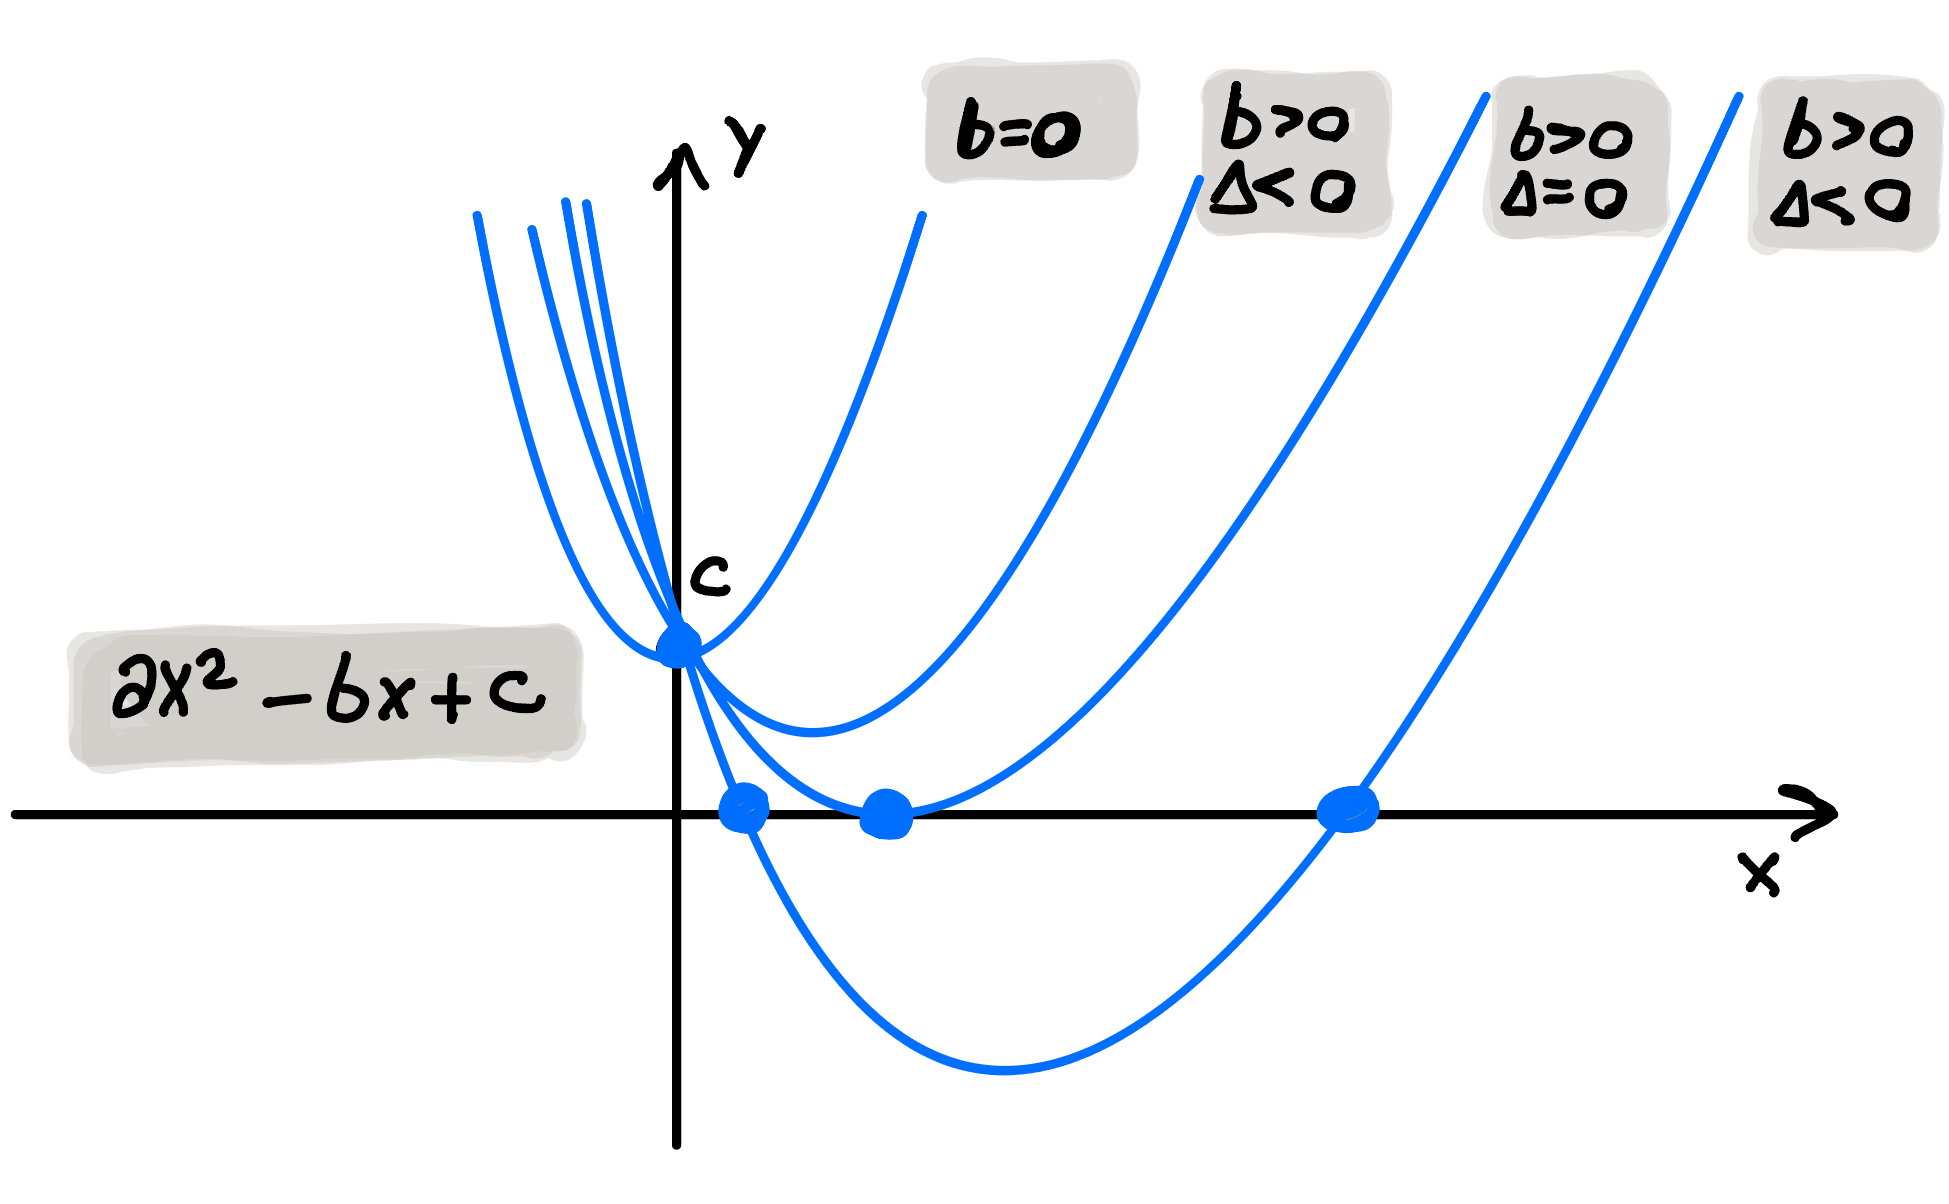
\includegraphics[width=\textwidth]{latex_source/images/turing/parable.jpeg}
\end{minipage}
\newline
We require:
\begin{equation*}
    \begin{cases}
        x_{min}(\epsilon,\,\sigma)>0 \\
        y_{min}(\epsilon,\,\sigma)\leq 0 \\
    \end{cases}
    \quad
        \begin{cases}
        \epsilon\,(g_v +\sigma\,f_u) > 0 \\
        [\epsilon\,(g_v +\sigma\,f_u)]^2 \geq 4\,\epsilon^2\,\sigma\,\text{det}[J] \\
    \end{cases}
\end{equation*} 
\noindent 
From the first one, one notices that there exists a minimum value threshold for $\sigma > \sigma_{min}= \frac{|g_v|}{f_u}$. Additionally, since $\text{tr}\,[J]=(-|g_v| +f_u)<0$, then $\sigma_{min}> 1$: a necessary condition for pattern initiation is that the inhibitor diffuses faster than the activator  (but it is still not sufficient). Proceeding,
\begin{equation*}
    \begin{cases}
        \sigma > \sigma_{min} >1  \\
        f_u^2\,\sigma^2 + 2\,(f_u\,g_v-2\,\text{det}[J])\,\sigma + g_v^2 \geq 0 
    \end{cases}
    \quad 
    \begin{cases}
    \sigma > \sigma_{min} >1  \\
    \sigma < \sigma_{-}(<\sigma_{min}) \quad \text{or} \quad  \sigma > \sigma_{+}\\
    \end{cases}
\end{equation*} 
where $\sigma_{\pm}$ are the roots of the quadratic equation:
\begin{equation*}
    \sigma_{\pm} = \frac{(f_u\,g_v - 2\,f_v\,g_u)\,\pm 2\,\sqrt{f_v\,g_u\,(f_v\,g_u-f_u\,g_v))}}{f_u^2}.
\end{equation*}
The function $y_{min}(\sigma)$ reaches its maximum for $\sigma=\sigma_{min}$ and goes to $-\infty$ for both $\sigma\rightarrow0^{+}$ and $\sigma\rightarrow +\infty$. Additionally, the lower-branch root $\sigma_{-}$ is below the threshold value $\sigma_{min}$. Then, both our requirements are satisfied if and only if $\sigma>\sigma_{+}$. In summary, the necessary and sufficient condition for instability is
\begin{equation*}
 \sigma > \sigma_c :=  \frac{(f_u\,g_v - 2\,f_v\,g_u)\, + 2\,\sqrt{f_v\,g_u\,(f_v\,g_u-f_u\,g_v))}}{f_u^2}
\end{equation*}
which is the critical threshold in [Eq: \ref{eq:critical_threshold}]. \bigskip \newline \noindent
\textbf{Critical eigenvalue and graph finite size effect} \newline
From the above equations, one also finds the critical eigenvalue $\Lambda_C$ [Eq: \ref{eq:critical_eigenvalue}] for given $\epsilon$:
\begin{equation*}
    \Lambda_c(\epsilon) \equiv x_{min}(\sigma_C,\,\epsilon)= \frac{g_v + \sigma_c\,f_u}{2\,\epsilon \,\sigma_c} = (\cdots) = \frac{1}{\epsilon}\,\sqrt{\frac{\text{det}[J]}{\sigma_c}}
\end{equation*}
When $\sigma > \sigma_C$ a range of $\Lambda$ values corresponding to unstable modes appears, centered around $\Lambda_c$. However, the eigenvalue spectrum of the laplacian matrix is not continuous: instability will be seen only if the network laplacian possesses at least one eigenvalue $\Lambda_n$ that falls inside this range.
In particular, the eigenvalue spectrum of the laplacian is bounded above for a graph of finite size: then, for $\epsilon$ sufficiently low, the critical eigenvalue could lay beyond the largest laplacian eigenvalue, $\Lambda_N$. In this case, no patterns would be seen. This finite-size effect is analogous to that found in a continuous medium.
\bigskip \newline
\textbf{Dispersion relation $\lambda(\Lambda;\, \sigma,\,\epsilon)$} \newline
Finally, the growing rate of the unstable mode, $\lambda_n = \lambda(\Lambda_n)$ is calculated from the caractheristic polynomial of $M(\Lambda_n, \sigma,\,\epsilon)$:
\begin{equation*}
    p(\lambda) = (\lambda-\lambda_1)\cdot(\lambda-\lambda_2) = \lambda^2 - \text{tr}[M(\Lambda,\,\sigma,\,\epsilon)]\cdot \lambda + \text{det}[M(\Lambda,\,\sigma,\,\epsilon)]
\end{equation*}
\begin{align*}
    \lambda_{\pm} &=\frac{1}{2}\,\left[\text{tr}[M]\pm \sqrt{\text{tr}[M]^2-4\,\text{det}[M]}\right] = \frac{1}{2}\,\left[-|\text{tr}[M]|\pm \sqrt{\text{tr}[M]^2-4\,\text{det}[M]}\right] \\
    &= \frac{1}{2}\, \left[\left[f_u + g_v - (1+\sigma)\,\epsilon\,\Lambda\right] \pm \sqrt{4\,f_v\,g_u + \left[f_u - g_v -(1-\sigma)\,\epsilon\,\Lambda\right]^2}\right]
\end{align*}
In the instability region, $\text{tr}[M] <0$ and $\text{det}[M]<0$, then eigenvalues are real and distinct. Also, the lower branch is always negative so we are not interested in it. 
\small}

\newpage